\PassOptionsToPackage{unicode=true}{hyperref} % options for packages loaded elsewhere
\PassOptionsToPackage{hyphens}{url}
\PassOptionsToPackage{dvipsnames,svgnames*,x11names*}{xcolor}
%
\documentclass[10pt,ignorenonframetext,]{beamer}
\usepackage{pgfpages}
\setbeamertemplate{caption}[numbered]
\setbeamertemplate{caption label separator}{: }
\setbeamercolor{caption name}{fg=normal text.fg}
\beamertemplatenavigationsymbolsempty
% Prevent slide breaks in the middle of a paragraph:
\widowpenalties 1 10000
\raggedbottom
\setbeamertemplate{part page}{
\centering
\begin{beamercolorbox}[sep=16pt,center]{part title}
  \usebeamerfont{part title}\insertpart\par
\end{beamercolorbox}
}
\setbeamertemplate{section page}{
\centering
\begin{beamercolorbox}[sep=12pt,center]{part title}
  \usebeamerfont{section title}\insertsection\par
\end{beamercolorbox}
}
\setbeamertemplate{subsection page}{
\centering
\begin{beamercolorbox}[sep=8pt,center]{part title}
  \usebeamerfont{subsection title}\insertsubsection\par
\end{beamercolorbox}
}
\AtBeginPart{
  \frame{\partpage}
}
\AtBeginSection{
  \ifbibliography
  \else
    \frame{\sectionpage}
  \fi
}
\AtBeginSubsection{
  \frame{\subsectionpage}
}
\usepackage{lmodern}
\usepackage{amssymb,amsmath}
\usepackage{ifxetex,ifluatex}
\usepackage{fixltx2e} % provides \textsubscript
\ifnum 0\ifxetex 1\fi\ifluatex 1\fi=0 % if pdftex
  \usepackage[T1]{fontenc}
  \usepackage[utf8]{inputenc}
  \usepackage{textcomp} % provides euro and other symbols
\else % if luatex or xelatex
  \usepackage{unicode-math}
  \defaultfontfeatures{Ligatures=TeX,Scale=MatchLowercase}
\fi
\usetheme[]{Singapore}
\usefonttheme{serif}
% use upquote if available, for straight quotes in verbatim environments
\IfFileExists{upquote.sty}{\usepackage{upquote}}{}
% use microtype if available
\IfFileExists{microtype.sty}{%
\usepackage[]{microtype}
\UseMicrotypeSet[protrusion]{basicmath} % disable protrusion for tt fonts
}{}
\IfFileExists{parskip.sty}{%
\usepackage{parskip}
}{% else
\setlength{\parindent}{0pt}
\setlength{\parskip}{6pt plus 2pt minus 1pt}
}
\usepackage{xcolor}
\usepackage{hyperref}
\hypersetup{
            pdftitle={ Statistical methods in quantitative genetics},
            pdfauthor={Stefanie Muff, CBD, Department of Mathematical Sciences, NTNU},
            colorlinks=true,
            linkcolor=Maroon,
            filecolor=Maroon,
            citecolor=Blue,
            urlcolor=blue,
            breaklinks=true}
\urlstyle{same}  % don't use monospace font for urls
\newif\ifbibliography
\usepackage{graphicx,grffile}
\makeatletter
\def\maxwidth{\ifdim\Gin@nat@width>\linewidth\linewidth\else\Gin@nat@width\fi}
\def\maxheight{\ifdim\Gin@nat@height>\textheight\textheight\else\Gin@nat@height\fi}
\makeatother
% Scale images if necessary, so that they will not overflow the page
% margins by default, and it is still possible to overwrite the defaults
% using explicit options in \includegraphics[width, height, ...]{}
\setkeys{Gin}{width=\maxwidth,height=\maxheight,keepaspectratio}
\setlength{\emergencystretch}{3em}  % prevent overfull lines
\providecommand{\tightlist}{%
  \setlength{\itemsep}{0pt}\setlength{\parskip}{0pt}}
\setcounter{secnumdepth}{0}

% set default figure placement to htbp
\makeatletter
\def\fps@figure{htbp}
\makeatother

\usepackage{multirow}

\title{
\includegraphics[width=1in,height=\textheight]{logo_ntnu.png}\\
Statistical methods in quantitative genetics}
\providecommand{\subtitle}[1]{}
\subtitle{Genetic group models and marker-based regression}
\author{Stefanie Muff, CBD, Department of Mathematical Sciences, NTNU}
\date{CAS Oslo, March 17 2020}

\begin{document}
\frame{\titlepage}

\begin{frame}

\begin{block}{Overview}

\vspace{3mm}

\begin{itemize}
\tightlist
\item
  Genetic group models

  \begin{itemize}
  \tightlist
  \item
    Differences in means
  \item
    Differences in additive genetic variance (VA)
  \end{itemize}
\end{itemize}

\vspace{2mm}

\begin{itemize}
\tightlist
\item
  Marker-based regression using genomic data
\end{itemize}

\end{block}

\end{frame}

\begin{frame}

\begin{block}{How I became an ecological statistician}

\vspace{3mm}

\begin{itemize}
\item
  Master in mathematics
\item
  PhD in computational structural biology
\item
  Certificate of Advanced Studies in applied statistics
\item
  Postdoc in medical and ecological statistics
\end{itemize}

\vspace{2mm}

Since Sept.~2019: Associate Professor in Statistics, CBD, Department of
Mathematical Sciences, NTNU Trondheim

\vspace{5mm}

I'm often not sure if I am

\vspace{2mm}

\begin{itemize}
\tightlist
\item
  a mathematician?
\item
  a biostatistician?\\
\item
  an ecological statistician?\\
\item
  an applied statistician?
\end{itemize}

\end{block}

\end{frame}

\begin{frame}

\begin{block}{Research interests}

\vspace{3mm}

\begin{itemize}
\tightlist
\item
  \emph{\textcolor{red}{Measurement error modeling}} (methods \&
  applications), see \emph{e.g.} Muff, Riebler, et al. (2015), Muff and
  Keller (2015), Muff, Puhan, and Held (2018).
\end{itemize}

\vspace{3mm}

\begin{itemize}
\tightlist
\item
  \emph{\textcolor{red}{Bayesian statistics}} (ideal for taming
  measurement errors!).
\end{itemize}

\vspace{3mm}

\begin{itemize}
\tightlist
\item
  \emph{\textcolor{red}{Quantitative genetics}}, see Ponzi et al.
  (2018), Ponzi, Keller, and Muff (2019), Muff, Niskanen, et al. (2019).
\end{itemize}

\vspace{3mm}

\begin{itemize}
\tightlist
\item
  \emph{\textcolor{red}{Movement ecology}}, see Weinberger et al. (2016)
  Gehr et al. (2017) or Muff, Signer, and Fieberg (2019).
\end{itemize}

\end{block}

\end{frame}

\begin{frame}{Part I: Genetic group animal models}
\protect\hypertarget{part-i-genetic-group-animal-models}{}

\begin{block}{The basic animal model}

\vspace{3mm}

\begin{itemize}
\tightlist
\item
  Given phenotypic measurements \(y_i\) for individuals
  \(1\leq i \leq n\), the most simple form of the animal model is \[
  y_i = \mu + a_i + e_i \ ,
  \] where \(e_i \sim \text{N}(0,\sigma_E^2)\) and
  \({\mathbf a}^\top = (a_1, \ldots, a_n)^\top \sim \text{N}({\mathbf a},\sigma_A^2 \mathbf{A})\)
  with additive genetic variance \(\sigma_A^2\) and additive genetic
  relatedness matrix \(\mathbf{A}\).
\end{itemize}

\vspace{3mm}

\begin{itemize}
\item
  The model can be extended by additional fixed or random effects.\\
  \vspace{3mm}
\item
  \textbf{Assumptions}:

  \begin{itemize}
  \tightlist
  \item
    All individuals derive from the same genetic population.
  \item
    The breeding values (\(a_i\)) encode for the deviation from the mean
    of this population and thus have an expected value
    \(\text{E}[a_i]=0\).
  \end{itemize}
\end{itemize}

\end{block}

\end{frame}

\begin{frame}

\begin{block}{Systematic deviation from the assumptions}

\vspace{3mm}

For example

\begin{itemize}
\tightlist
\item
  in cross-bred livestock.
\item
  when genetically different wild subpopulations mix (migration).
\end{itemize}

\centering

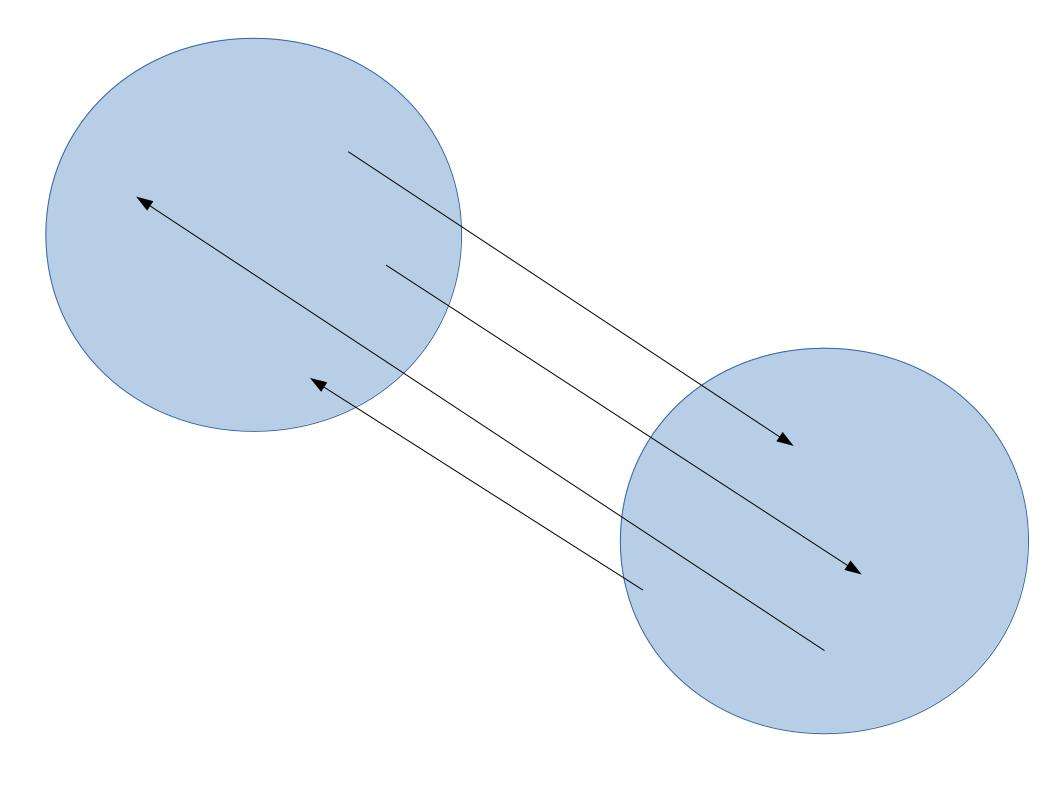
\includegraphics[width=0.5\textwidth,height=\textheight]{graphics/2populations.jpg}

\vspace{3mm}

\flushleft

\(\Rightarrow\) Individuals have a genetic origin that stems
\emph{\textcolor{red}{partially from both populations}}.

\vspace{2mm}

\textbf{Consequence}: Biased estimates of \(\sigma_A^2\) and breeding
values.

\end{block}

\end{frame}

\begin{frame}

\begin{block}{Genetic group models}

\vspace{3mm}

Great overview by Wolak and Reid (2017)

\vspace{2mm}

\center

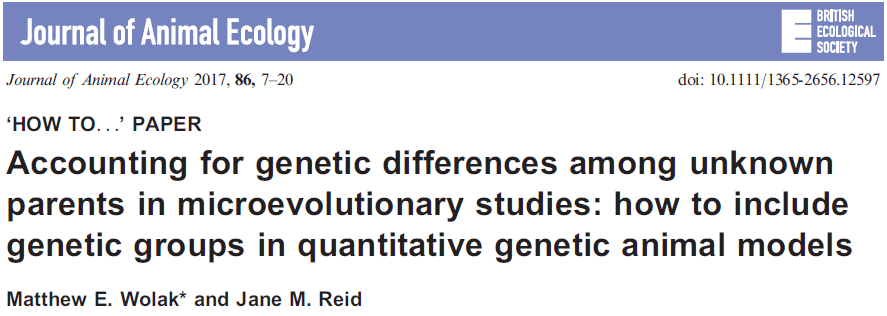
\includegraphics[width=0.8\textwidth,height=\textheight]{graphics/wolak_reid.png}

\vspace{3mm}
\vspace{3mm}

\flushleft

\textbf{Idea}: Allow for ``founder populations'' that differ in the
\emph{mean breeding value}.

\end{block}

\end{frame}

\begin{frame}

\begin{block}{Example for two isolated groups}

\vspace{3mm}

Simple model for a phenotypic trait \(y_i\) with mean \(\mu\), breeding
values \(a_i\) and environmental component \(e_i\): \vspace{-3mm}

\begin{align*} 
&\text{group 1:} \hspace{-14mm}  & y_i &= \mu +    \underbrace{a_i}_{u_i} +  e_i \ ,\\
&\text{group 2:}  \hspace{-14mm} & y_i &= \mu +  \underbrace{g_2 + a_i}_{u_i} +   e_i \ , 
\end{align*} \vspace{-3mm} thus

\[ u_i \sim \text{N}(0,\sigma_A^2 \mathbf{A})  \quad   \text{in group 1}. \]
\[ u_i \sim \text{N}(g_2,\sigma_A^2 \mathbf{A}) \quad     \text{in group 2}.\]
\vspace{3mm}

\begin{itemize}
\item
  \textbf{Interpretation:} The total additive genetic effects \(u_i\)
  (thus probably also the mean phenotypic values) differ between the two
  groups.
\item
  \textbf{Example:} Systematic differences in wing length,
  weight,\ldots{}
\end{itemize}

\end{block}

\end{frame}

\begin{frame}

General formulation of genetic group model with \(r\) groups \[
 y_i  = \mu + \underbrace{\sum_{j=1}^r q_{ij}g_j +  a_i}_{u_i} + e_i  \ , \quad \mathbf{a}^\top \sim \text{N}(\mathbf{0},\sigma_A^2\mathbf{A}) \ ,
\]

where \(0\leq q_{ij} \leq 1\) is the proportional
\emph{\textcolor{red}{contribution of group $j$ to the genome of individual $i$}}.

\vspace{3mm}
\vspace{3mm}

How do we obtain the \(q_{ij}\)?

\end{frame}

\begin{frame}[fragile]

\begin{block}{Example}

\vspace{3mm}

\begin{itemize}
\tightlist
\item
  Group 1: Founders nodes 1 and 2
\item
  Group 2: Founder node 3
\end{itemize}

\vspace{3mm}

\center

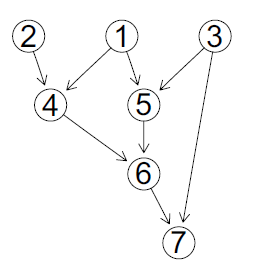
\includegraphics[width=0.3\textwidth,height=\textheight]{graphics/pedigree_GSE.png}
\hspace{6mm}
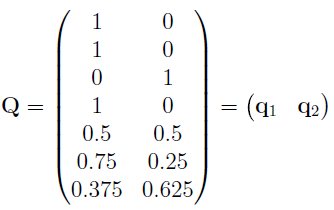
\includegraphics[width=0.45\textwidth,height=\textheight]{graphics/Q_GSE.png}

\vspace{10mm}

\flushleft

\small

\textbf{How to?} E.g. by using the \texttt{ggcontrib()} function from
the \texttt{nadive} R package (Wolak 2012).

\end{block}

\end{frame}

\begin{frame}

\begin{block}{Genetic group models for heterogeneous variances}

\vspace{3mm}

\begin{itemize}
\item
  \textbf{Caveat:} Additive genetic variances \(\sigma_A^2\) are assumed
  the same within the groups. \vspace{4mm}
\item
  \textbf{Idea}: Replace \begin{align*}
   y_i &= \mu + \sum_{j=1}^r q_{ij}g_j + \textcolor{red}{a_i}  +  e_i & (\text{homogeneous } \sigma_A^2) \quad\\ 
  \text{by} \\[2mm]
  y_i &= \mu + \sum_{j=1}^r q_{ij}g_j + \textcolor{red}{\sum_{j=1}^r a_{ij}}  +  e_i \ , & (\text{heterogeneous }  \sigma_{A_j}^2)  
  \end{align*} where
  \((a_{1j}, \ldots, a_{nj})^\top \sim \text{N}(0, \sigma_{A_j}^2 \mathbf{A}_j)\).
  \vspace{4mm}
\item
  \textbf{Two challenges}:

  \begin{enumerate}
  [1)]
  \tightlist
  \item
    Segregation variances between the groups.
  \item
    Finding the group-specific relatedness matrics \(\mathbf{A}_j\).
  \end{enumerate}
\end{itemize}

\end{block}

\end{frame}

\begin{frame}

Addressing these challenges was the purpose of this publication:

\center


\includegraphics[width=0.9\textwidth,height=\textheight]{graphics/GSE_paper.png}

\end{frame}

\begin{frame}

\begin{block}{Challenge 1: Segregation variances}

\vspace{3mm}

In principle, we would need to ``blow up'' our models with segregation
variances (e.g., García-Cortés and Toro
2006)\footnote{Segregation variance refers to the increase in variance caused by differences in allele combinations, average allelic effects, and linkage disequilibrium at and between loci underlying the phenotype in the mixing breeds}.
In our notation:
\[y_i = \mu + \sum_{j=1}^r q_{ij}g_j + \sum_{j=1}^r a_{ij}  + \sum_{j < k} s^{(jk)}_i +  e_i \ ,\]
\[\mathbf{s}^{(12)}\sim \text{N}(\mathbf{0},\sigma_{s_{12}}^2 \mathbf{A}_{12})  \ ,\]
thus we would need to estimate
\(r + \left( \begin{matrix} r\\ 2 \end{matrix}\right)\) variances.

\vspace{10mm}

\textbf{But is this relevant here?}

\end{block}

\end{frame}

\begin{frame}

\begin{itemize}
\tightlist
\item
  The segregation variance when crossing two genetic groups (e.g.,
  breeds) can be computed as
  \[\sigma_S^2 =\frac{1}{2} \sum_{i=1}^m (\alpha_i^c)^2 \ ,\] where
  \(\alpha_i^c\) denotes the mean additive genetic difference between
  the groups due to locus \(i\) (Lynch and Walsh, 1998), and \(m\) is
  the number of loci that determine the trait.
\end{itemize}

\vspace{3mm}

\begin{itemize}
\tightlist
\item
  Why can we often safely ignore \(\sigma_S^2\)?
\end{itemize}

\pause

\vspace{3mm}

\begin{block}{Under the \emph{infinitesimal model} assumption, all
\(\alpha_i^c\) are very small, and thus \(\sigma_S^2 \approx 0\).}

\end{block}

\end{frame}

\begin{frame}

\begin{block}{Challenge 2: Finding group-specific relatedness matrices
\(\mathbf{A}_j\)}

\vspace{3mm}

\begin{itemize}
\tightlist
\item
  First we recall: \(\mathbf{A}\) can be decomposed by a
  \emph{generalized Cholesky decomposition} into\\
  \[
  \mathbf{A} = \mathbf{T} \mathbf{D} \mathbf{T}' \ ,
  \] with lower triangular matrix \(\mathbf{T}\) and transposed
  \(\mathbf{T}'\), and diagonal matrix
  \(\mathbf{D}=\text{Diag}(d_{11},\ldots , d_{nn})\) (Henderson 1976).
\end{itemize}

\vspace{3mm}

\begin{itemize}
\tightlist
\item
  \(\mathbf{T}\) traces the flow of alleles from one generation to the
  other.
\end{itemize}

\vspace{3mm}

\begin{itemize}
\tightlist
\item
  The diagonal entries of \(\mathbf{D}\) scale the Mendelian sampling
  variance.
\end{itemize}

\end{block}

\end{frame}

\begin{frame}

\begin{block}{Example}

\vspace{3mm}

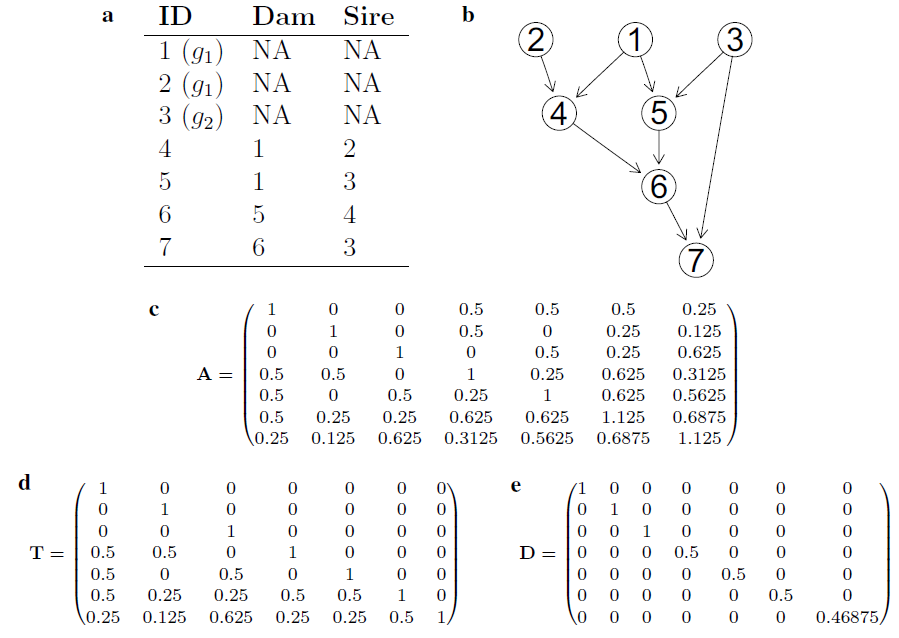
\includegraphics[width=0.9\textwidth,height=\textheight]{graphics/pedigree_matrices.png}

\end{block}

\end{frame}

\begin{frame}

\begin{block}{Basic idea}

\vspace{3mm}

Find \(\mathbf{A}_j\) by deriving group-specific versions
\(\mathbf{T}_j\) and \(\mathbf{D}_j\) and then use that

\[\mathbf{A}_j = \mathbf{T}_j \mathbf{D}_j \mathbf{T}_j ' \ .\]

\end{block}

\end{frame}

\begin{frame}

\begin{block}{Finding \(\mathbf{T}_j\)}

\vspace{3mm}

\begin{itemize}
\tightlist
\item
  \(T_j\) for group \(j\) represents the transmission of alleles through
  the generations \emph{within each group}.
\end{itemize}

\vspace{3mm}

\begin{itemize}
\tightlist
\item
  This can be obtained when we \emph{scale each row} of \(\mathbf{T}\)
  by \(\mathbf{q}_j\) or, equivalently, by
  \[\mathbf{T}_j = \mathbf{T} \cdot \text{Diag}(\mathbf{q}_j) \ , \] for
  diagonal matrix \(\text{Diag}(\mathbf{q}_j)\).
\end{itemize}

\end{block}

\end{frame}

\begin{frame}

\textbf{Toy-example:}

Given

\[\mathbf{T}  = \begin{pmatrix}
1 & 0 & 0\\
0.5 & 1 & 0 \\
0.25 & 0.5 & 1 \\
\end{pmatrix}\]

and a vector of group-membership proportions for group 1

\[\mathbf{q}_1 = \left( \begin{matrix} 1 \\ 0.5\\ 0  \end{matrix} \right) \ ,\]
we obtain

\[\mathbf{T}_1  =\mathbf{T} \cdot \text{Diag}(\mathbf{q}_1) =   \begin{pmatrix}
1 & 0 & 0\\
0.5 & 0.5 & 0 \\
0.25 & 0.25 & 0 \\
\end{pmatrix}\]

\end{frame}

\begin{frame}

\begin{block}{Finding \(\mathbf{D}_j\)}

\vspace{3mm}

\begin{itemize}
\tightlist
\item
  \textbf{Main finding}:

  \colorbox{lightgray}{\begin{minipage}{10cm}
  Given the entries $d_{ii}$ in the diagonal matrix $\mathbf{D}$, we get
  $$d^{(j)}_{ii} = 1 - q_{ij}(1-d_{ii}) \ .$$
  \end{minipage}}
\end{itemize}

\vspace{2mm}
\small

\begin{itemize}
\tightlist
\item
  Why? The original entries are \begin{equation*}
  d_{ii} = 
   \left\{\begin{array}{ll}
       1 \ , & \text{0 parent known},\\

       1-  0.25  - 0.25 (F_{p})\ , & \text{1 parent known},\\
       1 - 0.5 -  0.25 (F_{s} + F_{d}) \ , & \text{2 parents known}. \\
        \end{array}\right.
  \end{equation*} where \(F_p\), \(F_s\) and \(F_d\) are the
  pedigree-based inbreeding coefficients of the known parent(s).
\end{itemize}

\vspace{1mm}

\begin{itemize}
\tightlist
\item
  The group-specific versions \(d^{(j)}_{ii}\) are then obtained as
  \begin{equation*}
  d^{(j)}_{ii} =
  \left\{\begin{array}{ll}
       1 \ , & \text{0 parent known},\\
       1-  0.25 \cdot q_{ij}^{(p)} (1 + F_{p})\ , & \text{1 parent known},\\
       1 - 0.5 \cdot q_{ij} (1 +  \frac{F_{s} + F_{d}}{2}) \ , & \text{2 parents known}. \\
        \end{array}\right.
  \end{equation*}
\item
  Plus some algebraic rearrangements.
\end{itemize}

\end{block}

\end{frame}

\begin{frame}

\begin{block}{Caveat: \(\mathbf{D}_j\) is an approximation}

\(~\)

\begin{itemize}
\tightlist
\item
  This idea to find \(\mathbf{D}_j\) is an \emph{approximation}.
\end{itemize}

\(~\)

\begin{itemize}
\tightlist
\item
  Why? We assumed that parental inbreeding can be scaled by the genetic
  group proportions \(q_{ij}\).
\end{itemize}

\(~\)

\begin{itemize}
\tightlist
\item
  The correct way would be to use the actual
  \emph{\textcolor{red}{partial (i.e. group-specific) parental inbreeding coefficients}}
  \(F_s^{(j)}\) and \(F_d^{(j)}\), which capture inbreeding emerging
  \emph{within group \(j\)}.
\end{itemize}

\(~\)

\begin{itemize}
\tightlist
\item
  These can be obtained with some extra work, but we showed that
  approximations are \emph{\textcolor{red}{typically not critical}}.
\end{itemize}

\end{block}

\end{frame}

\begin{frame}

\begin{block}{Computations}

\vspace{3mm}

\begin{itemize}
\tightlist
\item
  Deriving \(\mathbf{T}_j\) and \(\mathbf{D}_j\) from \(\mathbf{T}\) and
  \(\mathbf{D}\) is cheap (simple algebraic transformations).
\end{itemize}

\vspace{3mm}

\begin{itemize}
\tightlist
\item
  The resulting \(\mathbf{A}_j\) are \emph{\textcolor{red}{singular}}.
  Replace 0's on the diagonal with a small value like \(10^{-6}\).
\end{itemize}

\vspace{3mm}

\begin{itemize}
\tightlist
\item
  All operations can also directly be carried out using
  \(\mathbf{A}^{-1}\).
\end{itemize}

\vspace{3mm}

\begin{itemize}
\tightlist
\item
  Models can be fitted with ingegrated nested Laplace approximations
  (INLA, Rue, Martino, and Chopin 2009) or MCMC (using e.g., MCMCglmm,
  Hadfield 2010).
\end{itemize}

\end{block}

\end{frame}

\begin{frame}

\begin{block}{Example: House sparrow system}

\vspace{2mm}

\begin{itemize}
\tightlist
\item
  House sparrow metapoplation at the Helgeland coast.
\end{itemize}

\vspace{2mm}

\begin{itemize}
\tightlist
\item
  Study running since 1993.
\end{itemize}

\vspace{2mm}

\begin{itemize}
\tightlist
\item
  Island-system can be broken up into three groups: \emph{inner},
  \emph{outer} and \emph{other} islands.
\end{itemize}

\vspace{3mm}

\center
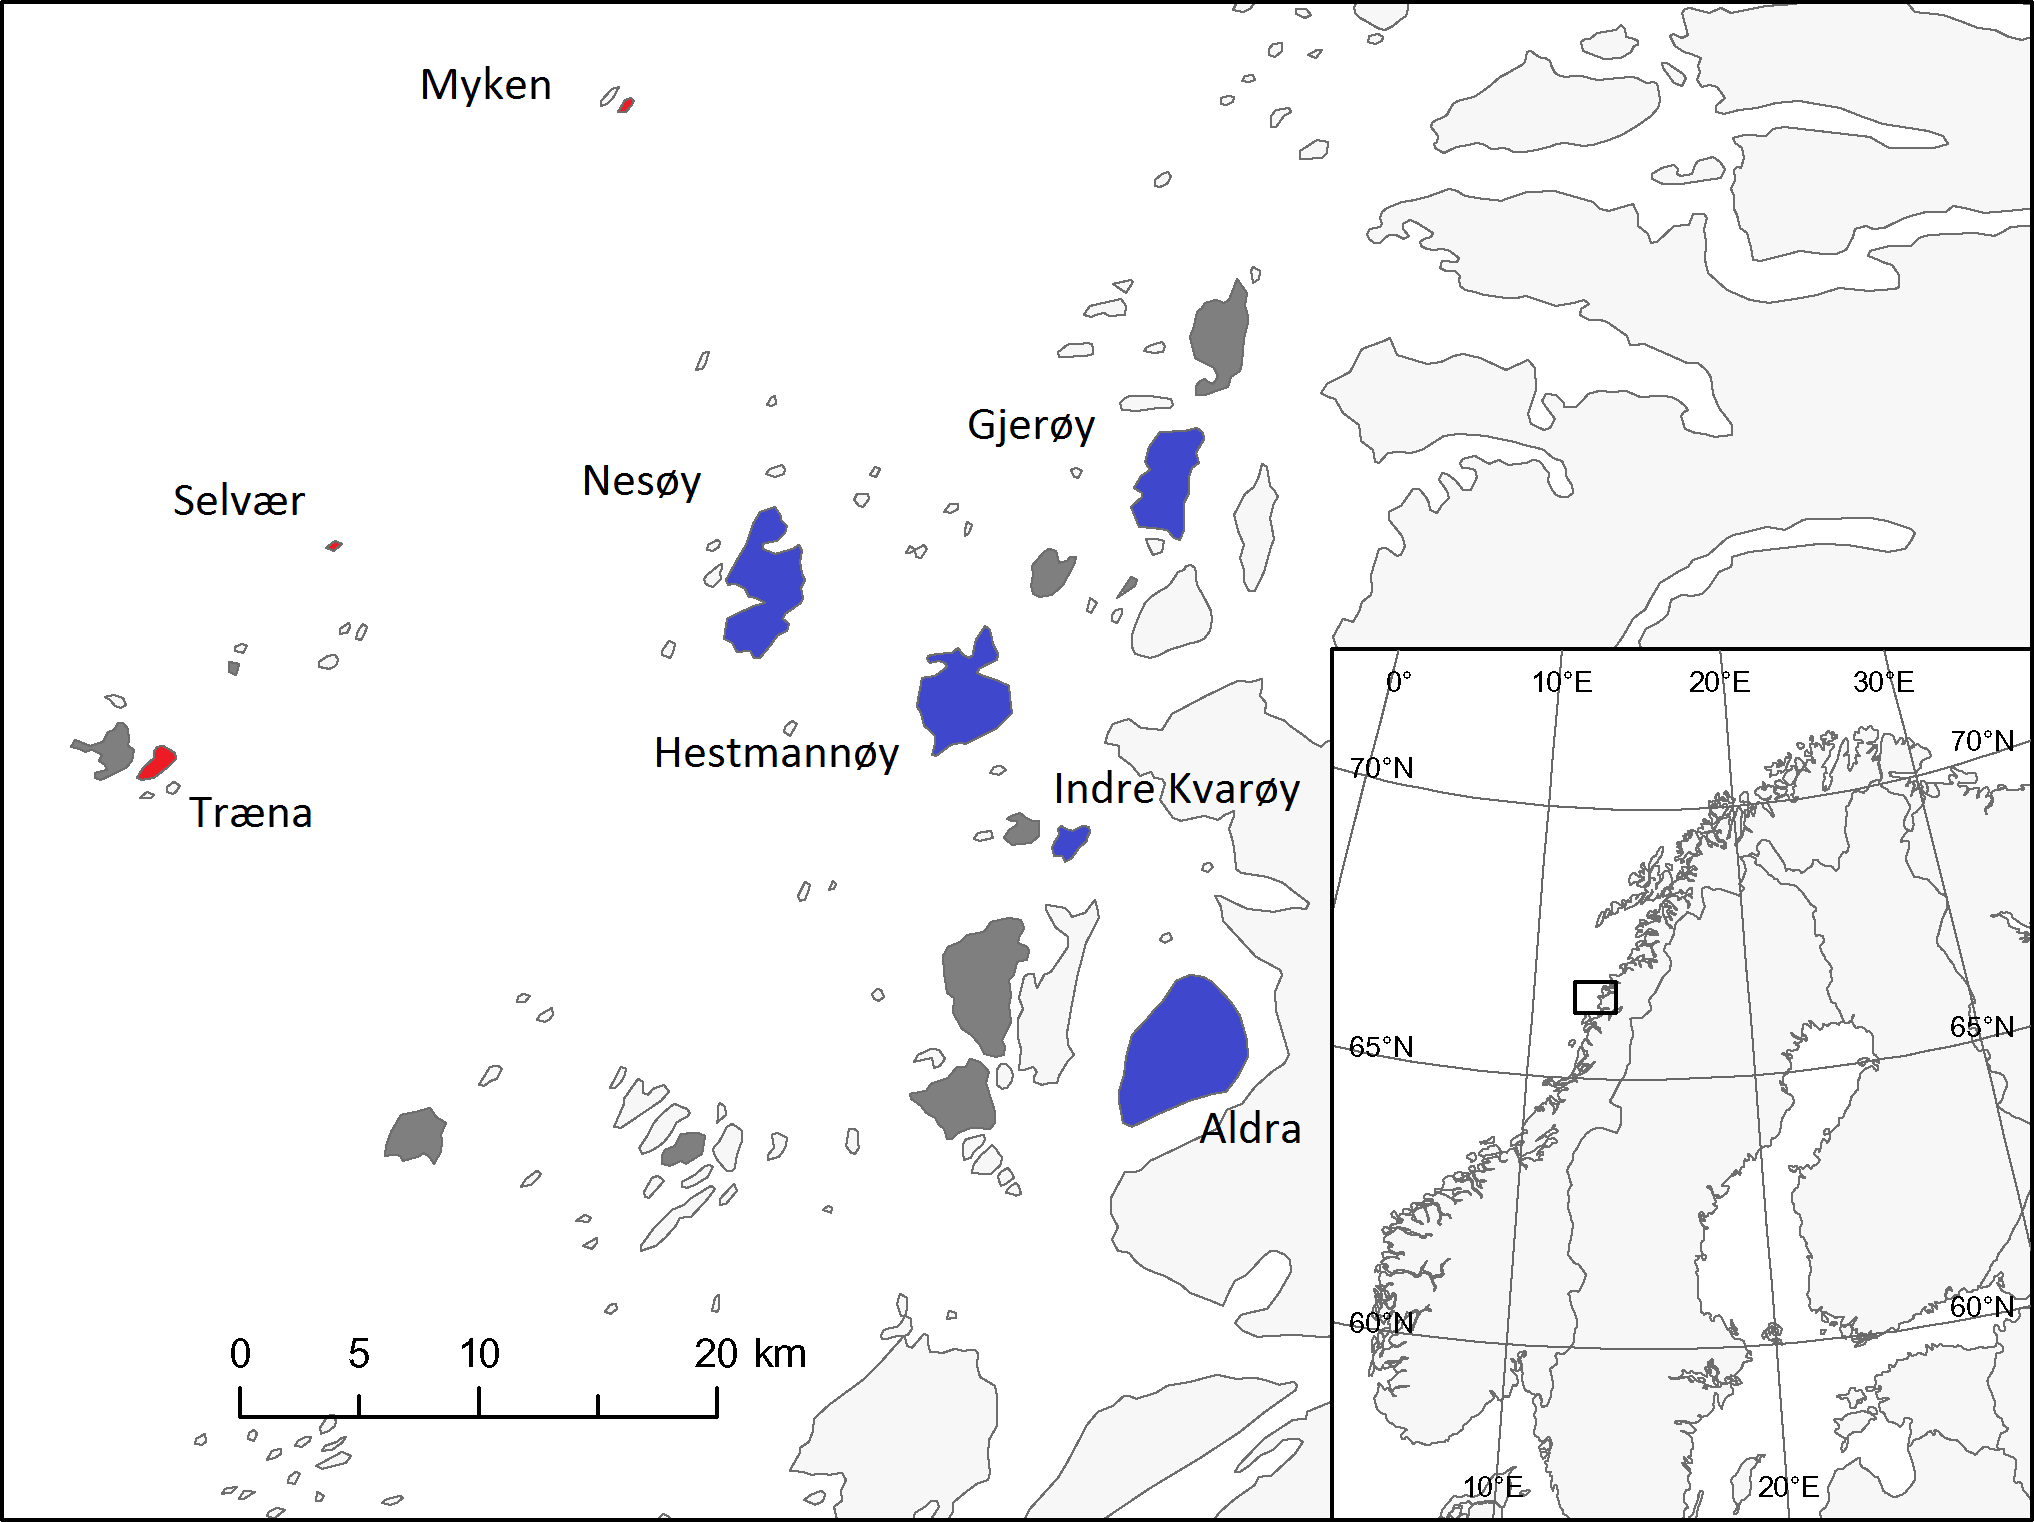
\includegraphics[width=0.6\textwidth,height=\textheight]{graphics/Helgeland.png}

\end{block}

\end{frame}

\begin{frame}{Part II: Marker-based regression}
\protect\hypertarget{part-ii-marker-based-regression}{}

\end{frame}

\begin{frame}{Acknowledgements}
\protect\hypertarget{acknowledgements}{}

\begin{itemize}
\item
  The Centre for Biodiversity Dynamics (CBD) and the research council of
  Norway (projects 221956 and 223257)
\item
  All my collaborators, in particular Henrik Jensen and Lukas F.~Keller
\item
  All the people that are collecting fantastic field data.
\end{itemize}

\end{frame}

\begin{frame}{References}
\protect\hypertarget{references}{}

\tiny

\hypertarget{refs}{}
\leavevmode\hypertarget{ref-garcia-cortes.etal2006}{}%
García-Cortés, Luis Alberto, and Miguel Ángel Toro. 2006. ``Multibreed
Analysis by Splitting the Breeding Values.'' \emph{Genetics Selection
Evolution} 38: 601--15.

\leavevmode\hypertarget{ref-gehr.etal2016}{}%
Gehr, B., E. Hofer, S. Muff, A. Ryser, E. Vimercati, K. Vogt, and L. F.
Keller. 2017. ``Spatial Scale and Behavioral State Interact in Shaping
Temporal Dynamics of Habitat Selection in Eurasian Lynx.'' \emph{Oikos}
126: 1389--99.

\leavevmode\hypertarget{ref-hadfield2010}{}%
Hadfield, J.D. 2010. ``MCMC Methods for Multi-Response Generalized
Linear Mixed Models: The MCMCglmm R Package.'' \emph{Journal of
Statistical Software} 33: 1--22.

\leavevmode\hypertarget{ref-henderson1976}{}%
Henderson, C.R. 1976. ``Simple Method for Computing Inverse of a
Numerator Relationship Matrix Used in Prediction of Breeding Values.''
\emph{Biometrics} 32: 69--83.

\leavevmode\hypertarget{ref-muff.keller2015}{}%
Muff, S., and L. F. Keller. 2015. ``Reverse Attenuation in Interaction
Terms Due to Covariate Error.'' \emph{Biometrical Journal} 57: 1068--83.

\leavevmode\hypertarget{ref-muff.etal2019}{}%
Muff, S., A.K. Niskanen, D. Saatoglu, L.F. Keller, and H. Jensen. 2019.
``Animal Models with Group-Specific Additive Genetic Variances:
Extending Genetic Group Models.'' \emph{Genetics, Selection, Evolution}
51:7.

\leavevmode\hypertarget{ref-muff.etal2018}{}%
Muff, S., M. A. Puhan, and L. Held. 2018. ``Bias Away from the Null Due
to Miscounted Outcomes?'' \emph{Statistical Methods in Medical Research}
27: 3151--66.

\leavevmode\hypertarget{ref-muff.etal2015}{}%
Muff, S., A. Riebler, L. Held, H. Rue, and P. Saner. 2015. ``Bayesian
Analysis of Measurement Error Models Using Integrated Nested Laplace
Approximations.'' \emph{Journal of the Royal Statistical Society. Series
C (Applied Statistics)} 64: 231--52.

\leavevmode\hypertarget{ref-muff.etal2019b}{}%
Muff, S., J. Signer, and J. Fieberg. 2019. ``Accounting for
Individual-Specific Variation in Habitat-Selection Studies: Efficient
Estimation of Mixed-Effects Models Using Bayesian or Frequentist
Computation.'' \emph{Journal of Animal Ecology} 89: 80--92.

\leavevmode\hypertarget{ref-ponzi.etal2018}{}%
Ponzi, E., L. F. Keller, T. Bonnet, and S. Muff. 2018. ``Heritability,
Selection, and the Response to Selection in the Presence of Phenotypic
Measurement Error: Effects, Cures, and the Role of Repeated
Measurements.'' \emph{Evolution} 72: 1992--2004.

\leavevmode\hypertarget{ref-ponzi.etal2019}{}%
Ponzi, E., L. F. Keller, and S. Muff. 2019. ``The Simulation
Extrapolation Technique Meets Ecology and Evolution: A General and
Intuitive Method to Account for Measurement Error.'' \emph{Methods in
Ecology and Evolution} 10: 1734--48.

\leavevmode\hypertarget{ref-rue.etal2009}{}%
Rue, H, S Martino, and N Chopin. 2009. ``Approximate Bayesian Inference
for Latent Gaussian Models by Using Integrated Nested Laplace
Approximations (with Discussion).'' \emph{Journal of the Royal
Statistical Society. Series B (Methodological)} 71: 319--92.

\leavevmode\hypertarget{ref-weinberger.etal2016}{}%
Weinberger, I. C., S. Muff, A. Kranz, and F. Bontadina. 2016. ``Flexible
Habitat Selection Paves the Way for a Recovery of Otter Populations in
the European Alps.'' \emph{Biological Conservation} 199: 88--95.

\leavevmode\hypertarget{ref-nadiv}{}%
Wolak, Matthew E. 2012. ``nadiv: An R Package to Create Relatedness
Matrices for Estimating Non-Additive Genetic Variances in Animal
Models.'' \emph{Methods in Ecology and Evolution} 3 (5): 792--96.
\url{http://onlinelibrary.wiley.com/doi/10.1111/j.2041-210X.2012.00213.x/full}.

\leavevmode\hypertarget{ref-wolak.reid2017}{}%
Wolak, Matthew E., and Jane M. Reid. 2017. ``Accounting for Genetic
Differences Among Unknown Parents in Microevolutionary Studies: How to
Include Genetic Groups in Quantitative Genetic Animal Models.''
\emph{Journal of Animal Ecology} 86 (1): 7--20.

\end{frame}

\end{document}
